\section{Introduction}

\mbox{}\\

The Leap Motion is the device that allows users to communicate with a master device using a set of gestures. The controller is based on two monochromatic IR cameras and infra red LEDs which allows it to detect movement within the range of 1 meter. Hands and gestures detected by the sensor are send as frames, around 200 per second, which are used later by the device program localised on the master device. Although the technology is being sold since 2012, the device is not working in a satisfying manner. Numerous problems may be found during usage, such as not detecting smaller hands, confusing left and right hand or misidentifying the extended fingers. \\

\paragraph{Problem specifications\\\\}

Considering above informations, the main aim of the project was to create an application, which, using newly designed gestures, would allow the user to communicate and control the robot arm. According to that, the main idea of the presented application is one of a writing robot, which could be used to write, draw or follow the user's hands on any surface, especially in hazardous and contaminated environment, which would not be safe or available for operator access. In order to correct the accuracy and quality of gesture recognition, additional mean filter has been applied.\\

To achieve the objectives, two individual modes were created. The first one, static mode, for detecting gestures which would correspond to a certain letter from the letters library. The second mode, based on dynamic detection of users' hand movement, which is followed by the robot's arm. \\

The application starts with mode selection, using the set of gestures presented in Figure \ref{fig:mode}, after which, the chosen mode is activated, but can be changed at any time of operating.


\begin{figure}[H]
	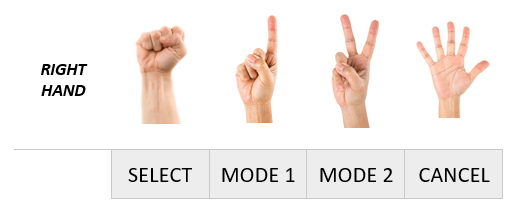
\includegraphics{mode_selection}
	\centering
	\caption{Mode selection - set of gestures}
	\label{fig:mode}
\end{figure}


The application is dedicated to be used with Universal Robot arm, which is easy to cooperate with and offers fast configuration, but could be applied to any similar working robot. Communication is realised by a certain part of the program, which will be described thoroughly in the following report. To allow most optimal and full application usage, the robot operation is realised by a set of functions written in C++, instead of programs dedicated to the robot.
